\solution{
\paragraph{Experimental setup.}
We fine-tuned \texttt{Qwen/Qwen2.5-0.5B} on a fixed, seeded subset of
1000 conversations from \texttt{HuggingFaceH4/ultrachat\_200k}'s
\texttt{train\_sft} split. We used 100 independently selected
\texttt{test\_sft} conversations for held-out loss and qualitative
evaluation. After seeded shuffling, we selected the first examples containing
an assistant target within the 512-token limit; skipped and selected identifiers
are provided with the immutable model and dataset revisions in
\texttt{results/sft/metadata.json} and
\texttt{results/sft/selection\_manifest.json}.

Each conversation was serialized in Qwen's ChatML format. Loss was applied
only to assistant content and end-of-message tokens; system and user tokens
were masked. Sequences were truncated to 512 tokens. All four variants used
two epochs, per-device batch size 4, four gradient-accumulation steps
(effective batch size 16), learning rate $5\times10^{-5}$, cosine decay,
3\% warm-up, AdamW, and BF16 arithmetic. LoRA targeted
\texttt{all-linear} with zero dropout and no bias. We set
$\alpha=2r$, keeping $\alpha/r=2$ constant so that rank was the intended
LoRA hyperparameter change.

\paragraph{Resource use and loss summary.}
\textbf{TODO after the Colab run: include the generated table below and
describe the trainable-parameter, peak-memory, runtime, and final-loss
differences.}

\begin{table}[t]
  \centering
  \begin{tabular}{lrrrrr}
\toprule
Method & Trainable params & Peak GiB & Time (min) & Mean train loss & Final val. loss \\
\midrule
LoRA r=1 & 549,888 & 12.70 & 2.66 & 1.4053 & 1.3879 \\
LoRA r=4 & 2,199,552 & 12.73 & 2.73 & 1.3889 & 1.3739 \\
LoRA r=16 & 8,798,208 & 12.79 & 2.75 & 1.3678 & 1.3648 \\
Full tuning & 494,032,768 & 15.26 & 2.66 & 1.1937 & 1.4123 \\
\bottomrule
\end{tabular}

  \caption{SFT resource use and final loss. Peak memory is the highest total
  device memory observed by polling \texttt{nvidia-smi} during
  \texttt{Trainer.train}. Training time includes its scheduled validation
  passes, but excludes model loading, the separate initial/final validation
  passes, and qualitative generation.}
  \label{tab:sft-resources}
\end{table}

\begin{figure}[t]
  \centering
  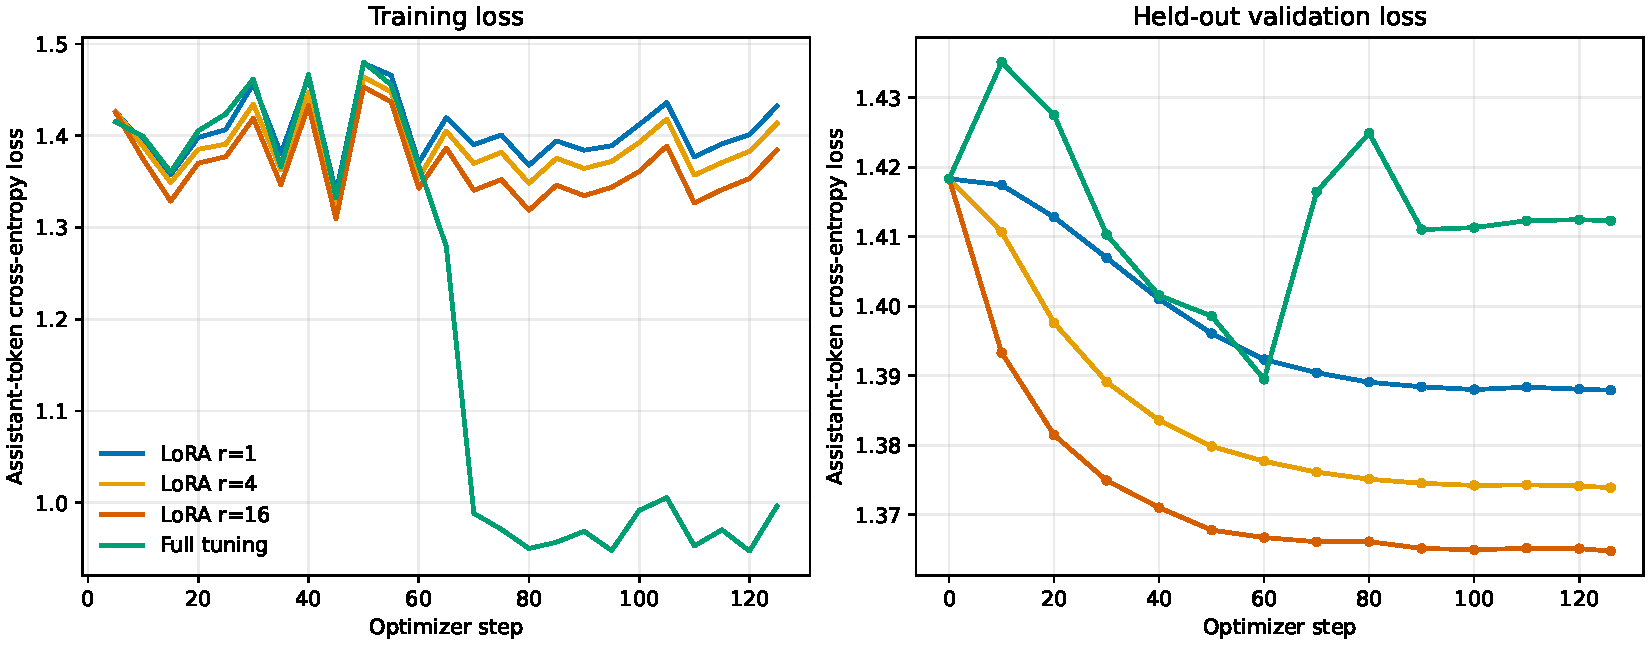
\includegraphics[width=0.98\linewidth]{figures/sft_loss_curves.pdf}
  \caption{Training loss (five-step logging windows) and held-out validation
  loss during SFT. All variants use identical examples, ordering, and
  evaluation intervals.}
  \label{fig:sft-losses}
\end{figure}

\begin{figure}[t]
  \centering
  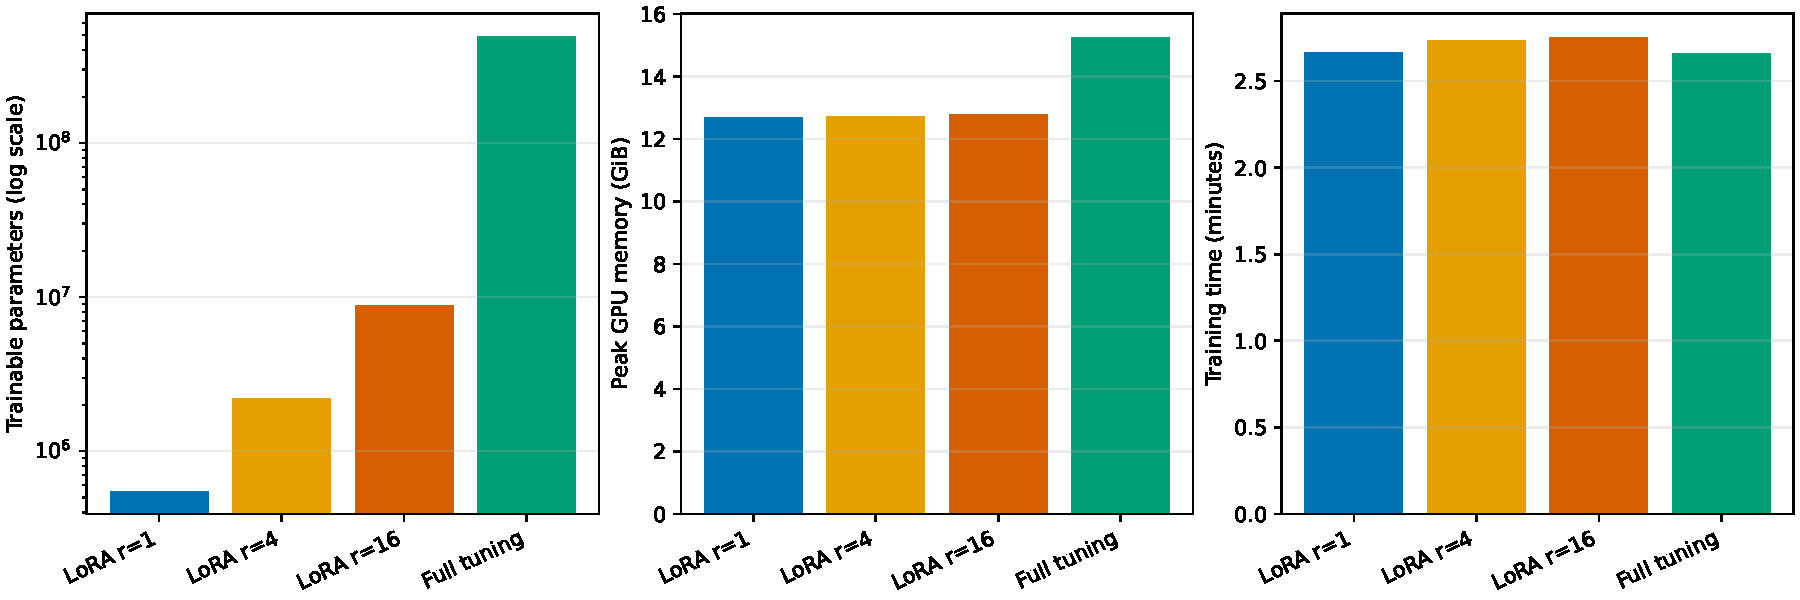
\includegraphics[width=0.98\linewidth]{figures/sft_resource_comparison.pdf}
  \caption{Trainable parameters, peak GPU memory, and training time for the
  three LoRA ranks and full-weight tuning.}
  \label{fig:sft-resources}
\end{figure}

\paragraph{Qualitative comparison.}
We greedily generated at most 128 tokens from the base model and every
fine-tuned variant for the same five held-out conversation prefixes. The
prompts, held-out reference responses, and unedited generations are listed in
\texttt{results/sft/qualitative\_generations.md}.

\textbf{TODO after the Colab run: discuss two or three concrete examples.}
Compare whether each model answers the requested instruction, adopts the
assistant role instead of continuing the user text, produces a coherent
conversational answer, and terminates with the expected message boundary.
Do not claim that a larger rank is better unless both the held-out losses and
the shown generations support that claim.

\paragraph{Artifacts.}
The experiment is implemented in
\texttt{scripts/sft\_experiment.py}; aggregation and plotting are implemented
in \texttt{scripts/plot\_sft\_results.py}. Raw loss history, resource metrics,
selection identifiers, metadata, and qualitative outputs are under
\texttt{results/sft/}.
}
